\documentclass[a4paper, 12pt, oneside]{article}
\usepackage{polski}
\usepackage[utf8]{inputenc}
\usepackage{geometry}
\usepackage{listings}
\usepackage{fancyhdr}
\usepackage{lastpage}
\usepackage{color}
\usepackage{graphicx}
\usepackage[hidelinks]{hyperref}
\newgeometry{tmargin=3.5cm, bmargin=3.5cm, lmargin=2.5cm, rmargin=2.5cm}
\linespread{2}

\title{\textbf{Projekt zaliczeniowy -- Timesheet}\linebreak Dokumentacja aplikacji do zarządzania zadaniami\linebreak}


\author{
Lider zespołu:\\
Jagoda Wykusz\\
\\
Pozostali członkowie:\\
Ryszard Białas,
Maksym Bielec,
Marcin Słota,
Oskar Ziomek\\
\linebreak}

\date{Uniwersytet Śląski\\2017}

\usepackage{fancyhdr}
 
\pagestyle{fancy}
\fancyhf{}
\rhead{Timesheet}
\lhead{\bfseries\leftmark}
\rfoot{str. \thepage /\pageref{LastPage}}

\begin{document}

% Strona tytułowa

\maketitle
\thispagestyle{empty}

\newpage

% Spis treści

\tableofcontents
\newpage

% Treść

\section{Założenia projektowe}
\paragraph{} W tym rozdziale opisane zostaną założenia, które przyświecały zespołowi podczas tworzenia aplikacji. Przedstawiony zostanie zarówno cel stworzenia programu, jak i funkcjonalności, które będą w nim docelowo dostępne.
	\subsection{Przeznaczenie aplikacji}
		\paragraph{}Celem niniejszego projektu jest stworzenie aplikacji webowej, pozwalającej na zarządzanie zadaniami podczas pracy w zespole. Umożliwiać ona będzie tworzenie wielu projektów, a w ich ramach zadań, do realizacji których przydzielać będzie można konkretnych użytkowników. Każdy projekt posiadać będzie menadżera, który ma większe uprawnienia, niż pozostali członkowie zespołu. Administrator aplikacji posiada maksymalne uprawnienia i może zarządzać również menadżerami.
		\paragraph{}Jednym z przykładów innych aplikacji podobnego rodzaju (choć w tym kontekście z nieco mniejszymi możliwościami), które są dostępne już na rynku, może być serwis Trello: \url{https://trello.com}.
	\subsection{Elementy składowe}
		\paragraph{}Zgodnie z przedstawionymi wymaganiami, tworzona aplikacja składać się będzie z następujących elementów (cech):
		\begin{itemize}
		
		\item Ogólne:
		
			\begin{itemize}
				\item Witryna internetowa,
				\item Należy zastosować ORM lub Micro-ORM,
				\item Dane powinny być walidowane po stronie front i back endu,
				\item Mechanizm logowania błędów,
				\item Projektu musi się znajdować na repozytorium,
				\item Dane muszą być zapisywane i odczytywane z bazy danych,
				\item Projekt będzie oceniany również ze względu na estetykę,
				\item Projekt musi posiadać czytelną dokumentację,
			\end{itemize}
			
		\item Aplikacja:
		
		\begin{itemize}
			\item Rejestracje nowego użytkownika wraz z podaniem danych osobowych,
			\item Mechanizm "Przypominania hasła",
			\item W systemie muszą występować 3 role - Administrator, Manager i Pracownik,
			\item Moduł przesyłania wiadomości pomiędzy użytkownikami systemu,
			\item We wszystkich tabelach w systemie powinna być możliwość filtracji danych,
			\item Należy zaimplementować mechanizm aprobowania wpisów.
		\end{itemize}
		
		\item Pracownik:
			\begin{itemize}
			
			\item Możliwość dodawania i edycji wpisów za danych dzień pracy. Wpis musi zawierać: datę, czas pracy, projekt, zadanie, komentarz,
			\item Wyświetlanie listy wszystkich wpisów (wraz z możliwością ich filtracji).
		
			\end{itemize}
			
			\item Manager:
			
			\begin{itemize}
			
			\item Wyświetlanie, dodawanie, edycja i usuwanie zadań (zadania powinny posiadać przewidywaną estymację),
\item Wyświetlanie wszystkich projektów, które są prowadzone przez danego managera,
\item Wyświetlanie listy pracowników w danym projekcie,
\item Generowanie raportu z przebiegu prac w projekcie,
\item Aprobowanie wpisów pracowników.
			
			\end{itemize}
			
			\item Administrator:
			
			\begin{itemize}
			
			\item Wyświetlanie listy użytkowników, zadań i projektów,
\item Możliwość zablokowania użytkownika lub wymuszenie zmiany hasła,
\item Dodawanie, edycja i usuwanie projektów,
\item Przypisywanie managerów i pracowników do projektów.
			
			\end{itemize}
			
			
			
		\end{itemize}
		
	\section{Specyfikacja techniczna}
	\paragraph{}W tym rozdziale opisane zostaną techniczne aspekty wykonania projektu, w tym zastosowane języki programowania, biblioteki oraz technologie. Zostanie również wyjaśniona kwestia zarządzania pracą w zespole, opisane repozytorium kodu oraz struktura bazy danych.
		\subsection{Język programowania i frameworki}
			\subsubsection{PHP oraz Laravel}
				\paragraph{} Aplikacja stworzona została w oparciu o skryptowy, interpretowany o język PHP. Od początku stosowano także framework Laravel w wersji 5.4 rozszerzający możliwości języka między innymi o modułowość. Framework ten rozwijany jest w marach licencji MIT. Jego kod źródłowy pozostaje dostępny w serwisie GitHub, pod adresem: \url{https://github.com/laravel}. Laravel uznawany jest za jeden z najpopularniejszych frameworków języka PHP. Szacuje się, iż wykorzystuje go obecnie kilkadziesiąt milionów aplikacji webowych.
			\subsubsection{Bootstrap}
				\paragraph{} Do stworzenia widoków w aplikacji wykorzystano framework Bootstrap. Gwarantuje on elementy zachowujące się zgodnie z ideologią RWD (Responsive Web Design) -- stron internetowych zachowujących responsywność w zależności od rozdzielczości ekranu, na którym wyświetlana jest witryna. Framework ten składa się z odpowiednio skonfigurowanych wstępnie plików CSS oraz JS, których dołączenie do projektu, a później tworzenie elementów interfejsu w oparciu o wspólne klasy, gwarantuje odpowiednie zachowanie strony.
				\paragraph{} W naszym projekcie elementy Bootstrapa zaimportowane zostały do projektu bezpośrednio z wzorca \textit{AdminLTE Control Panel Template} dostępnego w Internecie pod adresem: \url{https://adminlte.io}.  
				
		\subsection{Baza danych}
			\paragraph{}Na poniższym schemacie przedstawiono strukturę bazy danych wykorzystanej w projekcie:\\
			\linebreak
			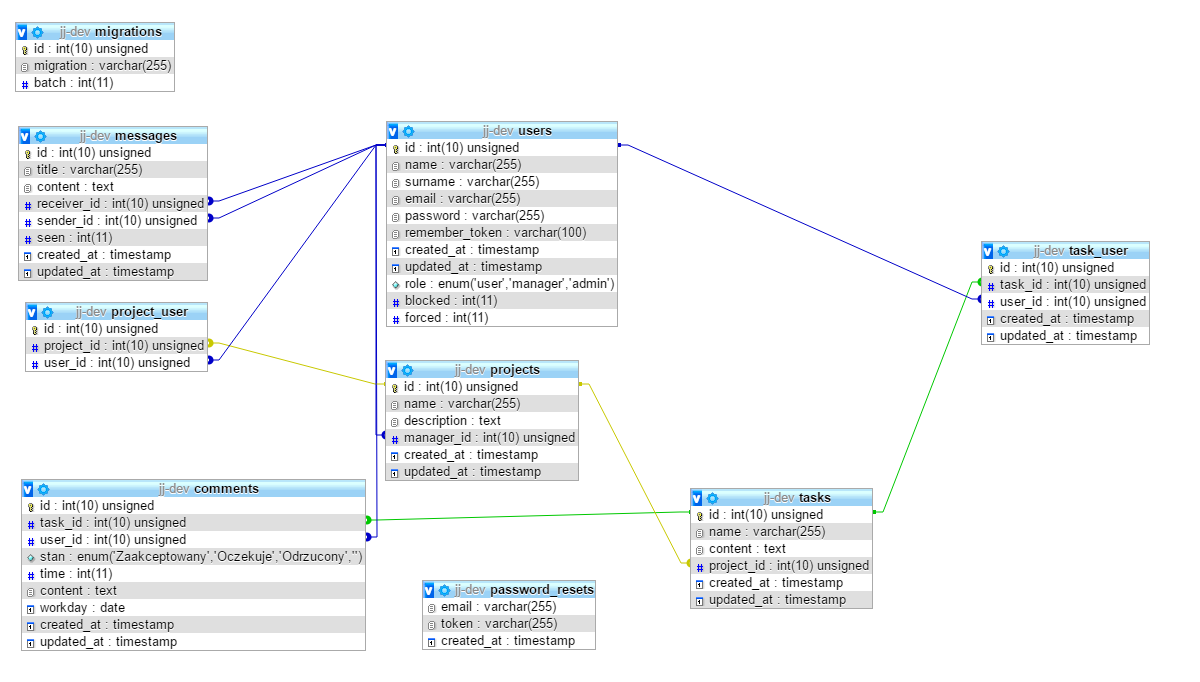
\includegraphics[width=17cm]{baza.png}
		\subsection{Repozytorium kodu}
			\paragraph{}Aby zapewnić najwyższą wygodę pracy w zespole oraz bezpieczeństwo tworzonego kodu aplikacji, pliki projektu umieszczone zostały w repozytorium w serwisie GitHub, pod adresem:  \url{https://github.com/Rys922/Timesheet}. Znajduje się tam najnowsza wersja kodu, która na bieżąco aktualizowana jest przez członków zespołu, wraz z postępem w pracach.
			\paragraph{} Wykorzystanie rozproszonego systemu kontroli wersji, jakim jest Git, gwarantuje dostępność kodu dla wszystkich członków zespołu i umożliwia jednoczesną pracę na plikach (aktualna wersja kodu zapisana jest zarówno lokalnie na komputerze programisty, jak i na głównym serwerze usługi).
			\subsection{Zarządzanie pracą w zespole}
			\paragraph{}Do rozdzielania prac pomiędzy członków zespołu tworzącego niniejszy projekt, wykorzystano serwis \textit{Trelloo} (\url{https://trello.com}). Jest to aplikacja pozwalająca dzielić zadania na grupy, przypisywać im osoby oraz wyznaczać terminy ich realizacji. Dzięki możliwości przenoszenia zrealizowanych zadań do innych grup, łatwo śledzić bieżący postęp w pracach. Pozwala to również w razie błędów cofnąć wybrany etap z fazy gotowości na przykład do fazy dalszych testów lub ponownej implementacji. 
		\subsection{Uruchomienie aplikacji}
			\paragraph{} Aby uruchomić aplikację na komputerze, konieczne jest jego wstępne skonfigurowanie. W przeciwieństwie do bazy danych, aplikacja nie została wdrożona na publiczny serwer, wobec czego niezbędne jest sklonowanie plików projektu z repozytorium, a następnie uruchamianie aplikacji lokalnie.
			\paragraph{}W tym celu konieczne jest pobranie aplikacji XAMPP (\url{https://www.apachefriends.org/pl}), a w niej uruchomienie modułu \textit{Apache}. Niezbędne jest również zmodyfikowanie dwóch plików konfiguracyjnych, by odpowiednio odwoływały się do tworzonej aplikacji:
			\begin{itemize}
				\item plik \verb+Windows\System32\drivers\etc\hosts+ należy uzupełnić o wpisy:
				\begin{footnotesize}
				\begin{lstlisting}[frame=single]  
127.0.0.1 timesheet.dev 
127.0.0.1 www.timesheet.dev
\end{lstlisting}
\end{footnotesize}
				\item plik \verb+xampp\apache\conf\extra\httpd-vhosts.conf+ należy uzupełnić o:
				\begin{footnotesize}
				\begin{lstlisting}[frame=single]  
<VirtualHost *:80>
  ServerName timesheet.dev
  ServerAlias www.timesheet.dev
  DocumentRoot "F:/xampp/htdocs/timesheet"
  <Directory "F:/xampp/htdocs/timesheet">
    AllowOverride All
    Order allow,deny
    Allow from all
  </Directory>
</VirtualHost>
\end{lstlisting}
\end{footnotesize}
			\end{itemize}
			
			\paragraph{}W drugim z powyższych przypadków należy zwrócić szczególną uwagę na ścieżkę, która musi odpowiadać faktycznej lokalizacji folderów XAMPP na dysku.
			
			\paragraph{}Kolejnym krokiem przed uruchomieniem aplikacji jest pobranie silnika frameworka i wypakowanie go w lokalizacji \verb+xampp\htdocs\timesheet\vendor+. Silnik ten udostępniliśmy do pobrania pod adresem: \url{https://www.dropbox.com/s/ceo3a3tkqdo8hsl/vendor.rar}.
			
			\paragraph{}Ostatnim etapem jest utworzenie pliku \verb+.env+ w głównym katalogu z plikami projektu, którego zawartość ma być następująca:\\
			
			\begin{footnotesize}
				\begin{lstlisting}[frame=single]  
APP_ENV=local
APP_KEY=base64:RFXLPxKbmADO9x167hZ5IkInLC0pAadBxWIBtQbt7Vg=
APP_DEBUG=true
APP_LOG_LEVEL=debug
APP_URL=http://www.timesheet.dev

DB_CONNECTION=mysql
DB_HOST=sql.jj-dev.nazwa.pl
DB_PORT=3306
DB_DATABASE=jj-dev
DB_USERNAME=jj-dev
DB_PASSWORD=Ancymony666

BROADCAST_DRIVER=log
CACHE_DRIVER=file
SESSION_DRIVER=file
QUEUE_DRIVER=sync

REDIS_HOST=127.0.0.1
REDIS_PASSWORD=null
REDIS_PORT=6379

MAIL_DRIVER=smtp
MAIL_HOST=mailtrap.io
MAIL_PORT=2525
MAIL_USERNAME=null
MAIL_PASSWORD=null
MAIL_ENCRYPTION=null

PUSHER_APP_ID=
PUSHER_APP_KEY=
PUSHER_APP_SECRET=
\end{lstlisting}
\end{footnotesize}
						
			
\section{Realizacja projektu}
	\paragraph{}W tym rozdziale przedstawione zostaną widoki ekranów, które dostępne są dla poszczególnych funkcji w tworzonej aplikacji. 
	\subsection{Zasada tworzenia widoków}
		Był sobie główny widok, który później się rozszerza
	\subsection{Wybrane widoki}
			\subsubsection{Główny ekran aplikacji}
			\subsubsection{Tworzenie nowego projektu}
			\subsubsection{Coś jeszcze (?)}
	\subsection{Mechanizm logowania użytkownika}
	\subsection{Mechanizm rejestracji użytkownika}
\section{Testowanie}
	\subsection{Metody testowania}
	\subsection{Jakieś wnioski?}
\section{Dalszy rozwój aplikacji}
	\subsection{Założenia, które nie zostały zrealizowane}
	\subsection{Możliwość rozbudowania aplikacji w przyszłości}
\end{document}